\documentclass[fontsize=12pt, paper=a4, headinclude, twoside=false, parskip=half+, pagesize=auto, numbers=noenddot, open=right, toc=listof, toc=bibliography]{scrreprt}
\usepackage[left=3cm, bottom=3cm, top=3cm]{geometry} % wenn es nicht anders geht sonst typearea (unten)
\usepackage{multirow} % Tabellen-Zellen über mehrere Zeilen
\usepackage{multicol} % mehre Spalten auf eine Seite
\usepackage{tabularx} % Für Tabellen mit vorgegeben Größen
\usepackage[automark]{scrpage2} % Kopf- und Fußzeilen
\usepackage[T1]{fontenc} % Ligaturen, richtige Umlaute im PDF 
\usepackage[utf8]{inputenc}% UTF8-Kodierung für Umlaute usw
\usepackage{bibgerm} % Bibliographie Umlaute in BibTeX
\usepackage{mathtools}

 
 \newcommand{\ourtitlepage}{
 %++++++++++++++++++++++++++++++++++++++++++++++++++++++++++++++++++
% Titelseite
%\clearscrheadings\clearscrplain
\begin{center}
{\large Universität Leipzig}\\
{\large Fakultät für Mathematik und Informatik}\\
{\large Institut für Informatik}\\
{\large Abteilung Automatische Sprachverarbeitung}\\
\vspace{5cm}
\begin{Large}
\textbf{Wortschatz Zeitgeist}\\
\vspace{5mm}
Seminararbeit\\
\vspace{5mm}
\end{Large}
\vspace{9cm}
\begin{tabular}{ r l }
{\bf Autoren:} 	& Döring, Thomas\\
			& Kießling, Max\\
			& Otto, Wolfgang (2885214)\\
{\bf Modul:} & Anwendungen Linguistische Informatik (10-202-2307)\\
{\bf Abgabe:} & {\today}. (Sommersemester 2015)\\
{\bf Betreuer:} & Maciej Janicki\\
{\bf Seminarleiter:}&Prof. Dr. Uwe Quasthoff\\ 
\end{tabular}\\
\end{center}
\clearpage

}


\begin{document}
\ourtitlepage 
\tableofcontents
\clearpage
\pagenumbering{arabic} % ab jetzt die normale arabische Nummerierung
\chapter{Einleitung}
\section{Aufgabenstellung}
Es soll untersucht werden, welche Maße sinnvoll für die Generierung der Wörter des Tages sind. Eine Implementierung soll in SQL und für Zeitreihenuntersuchungen in R erfolgen.\\
Desweiteren soll ein regelbasiertes Verfahren implementiert werden um Datumsangaben und andere strukturelle Worte zu filtern.\\
\section{Status quo}
\section{Vergleichbare Ansätze}
Tagesaktuelle Wikiartikel\\
google trends?\\


\chapter{Das finden von Tagesaktuellen Wörter}
\section{Maße zur Trend-Detection}
\subsection{Relatives Vorkommen (Referenz)}
Das Maß wird durch die Differenz des relativen Anteils eines Tokens an allen Tokens eines Tages und dem relativen Anteil eines Tokens an allen Tokens eines Vergleichskorpus bestimmt. 
\begin{equation}
sig_{referenz}(w) = p_{tag} - p_{jahr}
\end{equation}

\subsection{Poisson-Maß}

Die Formel leitet sich aus der Poissonverteilung ab und beschreibt wie Wahrscheinlich es ist, dass die gemessene Tagesfrequenz beobachtet werden kann. 
\begin{equation}
sig_{poisson}(w) = \frac{k(\log(k)-\log(n\cdot p) -1 ))}{\log(n)}
\end{equation}
k:= Anzahl der Token von w in Tagesbericht\\
n := Anzahl der Tokens in Tagesbericht\\
p := relativer Anteil eines Tokens am Jahreskorpus\\
Es ist das gleiche Maß wie in \cite[S. 338-340]{heyer06} beschrieben und hergeleitet. Hier aber nicht zum auffinden von signifikanten Kookurenzen, sondern zum auffinden von signifikanten Nennungen im Tageskorpus gegenüber einem Vergleichskorpus.\\

\subsection{Termfrequenz inverse Dokumentenfrequenz (tf-idf)}
 \begin{equation}
sig_{tf idf}(w) = \frac{k}{\max(K)} \cdot \log ( \frac{365}{|documentdays(w)|})
\end{equation}

\subsection{Z-Score}
Benattar et al. beschreiben in \cite{benattar2011trend} einen Ansatz zur Trend-Erkennung basierend auf dem Z-Score. Dabei beziehen Sie neben der relativen Worthäufigkeit noch die Anzahl der Tage ein an denen ein Wort mindestens einmal auftritt, um so das 0-Frequenz-Problem zu umgehen.

\subsubsection{Berechnung}
\begin{itemize}
	\item{Wortfrequenz}\\
		$f(w)_d :=$ Anzahl der Vorkommen von Wort $w$ an Datum $d$
	\item{relative Worthäufigkeit}\\
		Die relative Worthäufigkeit $p(w)_d$ berechnet sich durch: \\
		$t_d :=$ Anzahl verschiedener Worte an Datum $d$
		$$ p(w)_d = \frac{f(w)_d}{t_d} \\ $$
	\item{Erwartungswert}\\
		Der Erwartungswert $\bar{w}$ berechnet sich durch: \\
		$N:=$ Anzahl der Tage in der betrachteten Zeitspanne
		$$\bar{w}=\frac{1}{N} \sum p(w)_d$$
	\item{Standartabweichung}\\
		Die Standartabweichung $\sigma_w$ berechnet sich durch:
		$$\sigma_w = \sqrt{\frac{1}{N} \sum (p(w)_d - \bar{w}^2}$$
	\item{ZScore}\\
		Der Zscore $Z(w)_d$ misst die Abweichung der relativen Worthäufigkeit vom Erwartungswert in Vielfachen der Standartabweichung.
		$$Z(w)_d= \frac{p(w)_d - \bar{w}}{\sigma_w}$$		
	\item{Auftrittshäufigkeit}\\
		Die Auftrittshäufigkeit $Po(w)$ gibt an wie vielen Tagen innerhalb des betrachteten Zeitraums das Wort mindestens einmal auftritt:\\
		$nbD(w) :=$ Anzahl der Tage an denen $w$ vorkommt//
		$c_d:=$ Anzahl der Tage innerhalb des betrachteten Zeitraums
		$$Po(w)=\frac{nbD(w}{c_d}$$
	\item{Schwellwerte}
		Zur besseren Unterscheidung echter Trends von statistischen Anomalien schlagen Benattar et. al. vor die Worte anhand ihrer Auftrittshäufigkeit zu clustern. Den Clustern werden dabei Z-Score-Schwellwerte zugeordnet. Überschreitet der Z-Score eines Wortes den Schwellwert seines Clusters wird dieses Wort als signifikant und somit als Trend eingestuft. Cluster mit niedriger Auftrittshäufigkeit erhalten dabei höhere Schwellwerte. Je häufiger ein Wort auftritt desto niedriger wird der Schwellwert. 
		
		
\end{itemize}

\subsubsection{Vorgehen}
\begin{enumerate}
	\item Für jedes Wort in $w$ in $d$ berechne $Z(w)$
	\item 
\end{enumerate}




\subsection{Weitere Maße}
Einbeziehung der Anzahl von Quellen.

\section{Zeitreihenanalysen}
\section{Cleaning}
Es sollen Datumsangaben und evtl. neu auftauchende strukturelle Angaben ausgefiltert werden.\\
Ansatz: Regelbasiert.\\
Gibt es Maße, die solche Angaben strukturell ausschließen?


\chapter{Implementierungen in SQL und R}
\chapter{Ein empirischer Vergleich}
 
Kriterien: Anteil niederfrequenter Wörter in der Top-Liste\\
\section{Einleitung}
Die Messung der G\"ute der Ergebnisse stellt eine Herausforderung dar, da es keine geeignete Referenz, beispielswiese in Form eines Goldstandards der wichtigsten Worte eines Tages gibt. Um die G\'ute trotzdem einsch\"atzen zu k\"onnen bieten sich zwei herangehensweisen an. Zum einen die eigenst\"andige manuelle Pr\"ufung der Ergebnisse unter selbst formulierten Kriterien, zum anderen der quantitative Vergleich mittels eines geeigneten Abstandsma\ss es. Letzterer Ansatz bietet aber nur die M\"oglichkeit eines Verlgeiches der \"Ahnlichkeiten der Ergebnisse und hilft abzusch\"atzen wie sich die Ergebnisse gegeneinander verhalten. \"Uber die G\"ute gibt diese Methode keine Auskunft. Allerdings lassen sich Ausrei\ss er gut erkennen und der Pr\"amisse, dass gleiche Ergebnisse, die aus verschiedenen M\"ass ungen stammen eine h\"ohere Wahrscheinlichkeit besitzen gute Ergebnisse zu sein l\"asst sich auch die Qualit\"at beurteilen.
\section{Qualitativer Vergleich}
Um sich einen Eindruck der Ergebnisse anhand der resultierenden soriterten Wortlisten zu verschaffen wurden die Listen ausgew\"ahlter Tage verglichen. Da die Untersuchenden keine ausgewiesene Expertiese ausweist, die wichtigsten W\"orter eines t\"aglichen Nachrichtenstroms zu indentifizieren, die \"uber der eines Zeitungslesers liegt kann die Analyse nicht in die Tiefe gehen. Aber durch die Wahl der Tage l\"asst sich das \"Uberblicken der Ergebnisse vereinfachen. Deshalb w\"ahlten wir den 1.1.2015. \\
 Das funktiuoniert so noch nicht!!! Umschreiben ist nur blabla!!
\section{Quantitativer Vergleich - Average Overlap als Vergleichma\ss}
\subsection{Einf\"uhrung}
Der Vergleich zweier mit einer Rangfolge versehenen Listen ist ein bekanntes Problem. In unserem Fall handelt es sich um den spezialfall von Listen gleicher und fester L\"ange, aber einer potentiell unendlichen Zahl verschiedener W\"orter. Desweiteren sind die Listen nicht \emph{Conjoint}, was bedeutet, dass nicht nur gemeinsame W\"orter in den verschiedenen Listen auftauchen. In \cite{webber2010similarity} werden als Einleitung f\"ur ein Ma\ss, dass in der Lage ist auch unendliche Listen und Listen verschiedener L\"ange vergleichen zu k\"onnen geeignete Verfahren vorgestellt um solche Listen zu vergleichen. Das gew\"ahlte Verfahren \emph{Average Overlap} wird von den Autoren als \emph{top-k ranking} identifiziert. Also ein Ranking bis zu einer definierten Tiefe von k.\\
Der Vorteil des genutzten Verfahrens f\"ur unseren Anwendungsfall ist, dass der Rang der W\"orter einen Einfluss auf das Ma\ss haben. \"Ahnlichkeiten an der Spitze der Liste werden st\"arker gewichtet.\\
Das Verfahren ist ein Mengenbasierter Ansatz. Listen sind sich dann \"ahnlich, wenn sie die relative Anzahl gemeinsamer W\"orter hoch ist. Um nun aufsteigende Gewichtungen zu erhalten wird nun nicht nur die gesamte \"Uberlappung zweier Listen gemessen, sondern die Listen in K Listen unterteilt, wobei K die L\"ange der Listen ist und jede einzelne Liste jeweils alle Elemente bis zu dem Rang des Laufindexes k von 1 bis K enth\"alt. Also eine Liste der Form: [[ Wort 1],[Wort 1, Wort 2], ...]. Nun wird bei den einzelnen Listen gleicher L\"ange die relative \"Uberlappung gemessen. Um nun das Verlgleichsma\ss  zu erhalten wird der Durchschnitt aller errechneten Werte gemessen.  Formalisiert ergibt dies.
\begin{equation}
AO(S,T) = \frac{\sum_{k=1}^K\frac{| M(S_k) \cap M(T_k)|}{k}}{K}
\end{equation}
Wobei $S$ und $T$ zwei Listen sind, der tiefgestellte Index $k$ die Teilliste bis zum Rang $k$ angibt und $K$ die L\"ange der beiden Listen definiert. $M$ ist hierbei die Abbildung einer Liste auf die Menge der enthaltenen Elemente.\\
%Beispiel:\\
\subsection{Ergebnisse}
Hier die Ergebnisse
\begin{table}[ht]
\centering
\begin{tabular}{rllr}
  \hline
 & source & target & value \\ 
  \hline
1 & tf\_idf & poisson & 0.66 \\ 
  2 & tf\_idf & z-score & 0.18 \\ 
  3 & tf\_idf & freqratio & 0.31 \\ 
  4 & tf\_idf & freqratio\_old & 0.31 \\ 
  5 & tf\_idf & poisson\_old & 0.66 \\ 
  6 & poisson & z-score & 0.15 \\ 
  7 & poisson & freqratio & 0.16 \\ 
  8 & poisson & freqratio\_old & 0.16 \\ 
  9 & poisson & poisson\_old & 1.00 \\ 
  10 & z-score & freqratio & 0.16 \\ 
  11 & z-score & freqratio\_old & 0.16 \\ 
  12 & z-score & poisson\_old & 0.15 \\ 
  13 & freqratio & freqratio\_old & 1.00 \\ 
  14 & freqratio & poisson\_old & 0.16 \\ 
  15 & freqratio\_old & poisson\_old & 0.16 \\ 
   \hline
\end{tabular}
\caption{Avarage Overlap Comparison} 
\label{AvarageOverlapComparison}
\end{table}
\begin{figure}[htbp] 
  \centering
     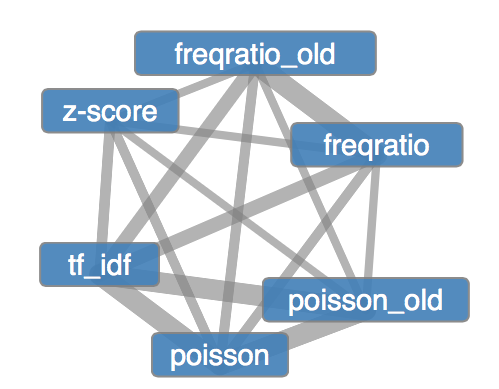
\includegraphics[width=0.7\textwidth]{pictures/comparison.png}
  \caption{Graph of Average Overlap}
  \label{fig:comparisonGraph}
\end{figure}
 


\chapter{Bewertung und Zusammenfassung}











 
\nocite{*}%alle nicht aufgeführte Literatur auch auffuehren
\bibliographystyle{plaindin} %alphadin_martin
\bibliography{wortschatzZeitgeistLit} 


\end{document}